\documentclass[10pt,twocolumn]{article}

\usepackage{geometry}
\geometry{margin=2cm}
\usepackage{amsmath,amsfonts,amssymb}
\usepackage{graphicx}
\usepackage{booktabs}
\usepackage{hyperref}
\usepackage{xcolor}
\usepackage{algorithm}
\usepackage{algpseudocode}
\usepackage{caption}
\usepackage{subcaption}
\usepackage{multirow}
\usepackage{array}
\usepackage{tikz}
\usetikzlibrary{arrows.meta, positioning, fit, calc}

\hypersetup{
  colorlinks=true,
  linkcolor=blue!60!black,
  citecolor=blue!60!black,
  urlcolor=blue!60!black
}

\title{\textbf{Silicon-Verified Two's Complement Floating-Point\\Arithmetic on FPGA}}
\author{Nick Spiker}
\date{}

\begin{document}

\twocolumn[
\maketitle
\begin{abstract}
We present a silicon-verified FPGA implementation of a two's complement
floating-point arithmetic system and compare it against two established
IEEE~754 libraries---Berkeley HardFloat and ETH Z\"urich FPnew (CVFPU)---on
identical hardware.  The system represents numbers as signed two's complement
fractions with unbiased signed exponents, eliminating the sign-magnitude
decomposition and biased exponent arithmetic of IEEE~754.  We implement
addition/subtraction, multiplication, and fused multiply-add (FMA) at
binary32-equivalent precision (25-bit fraction, 8-bit exponent) and
measure maximum operating frequency on a Lattice ECP5-25F using a
clock-enable-gated self-test harness that provides true silicon Fmax
rather than static timing estimates.

Results show that the two's complement approach achieves higher operating
frequency and lower area than both HardFloat and FPnew across all three
operations.  With DSP blocks enabled: addition runs at 95~MHz in 618~LUT4
(vs.\ HardFloat 88~MHz / 1050~LUT4), multiplication at 115~MHz in 157~LUT4
with 3~DSP (vs.\ 65~MHz / 786~LUT4 / 4~DSP), and FMA at 63~MHz in
1128~LUT4 with 3~DSP (vs.\ 47~MHz / 2057~LUT4 / 4~DSP).  Without DSP
blocks: addition 95~MHz / 618~LUT4 (vs.\ FPnew 74~MHz / 825~LUT4),
multiplication 95~MHz / 1750~LUT4 (vs.\ 74~MHz / 2850~LUT4), and FMA
53~MHz / 2768~LUT4 (vs.\ 25~MHz / 2850~LUT4).
\end{abstract}
\vspace{1em}
]

% ===========================================================================
\section{Introduction}
% ===========================================================================

IEEE~754 floating-point arithmetic has been the universal standard since
1985, yet its sign-magnitude representation with biased exponents introduces
implementation complexity that translates directly into silicon area and
critical-path depth.  Every arithmetic operation must decompose sign from
magnitude, handle sign combinations via conditional logic, and reconstruct
the result---a process that particularly penalizes operations like addition
where operand signs determine whether the underlying operation is addition
or subtraction.

We describe an alternative floating-point system, \emph{Spirix}, that uses
two's complement representation throughout the entire datapath.  Numbers are
represented as a signed two's complement fraction (the \emph{significand})
paired with an unbiased signed two's complement exponent:
\begin{equation}
  v = \frac{f}{2^{n-1}} \times 2^{e}
\end{equation}
where $f$ is an $n$-bit signed fraction and $e$ is an $m$-bit signed
exponent.  This eliminates the sign bit, the implicit leading one, the
exponent bias, and the separate handling of positive and negative zero.

The system uses \emph{N-1 normalization}: the two most significant bits of
a normal fraction always differ (\texttt{01...} for positive, \texttt{10...}
for negative), analogous to IEEE's implicit leading one but naturally
encoding sign.  A single reserved exponent value $e_{\min} = -2^{m-1}$
(the ``ambiguous exponent'') encodes all non-normal states: zero, infinity,
overflow (``exploded''), underflow (``vanished''), and undefined results.

This paper focuses on the hardware implementation: we present combinational
and pipelined arithmetic units for addition, multiplication, and fused
multiply-add at binary32-equivalent precision, and compare them against
Berkeley HardFloat~\cite{hardFloat} and ETH Z\"urich FPnew~\cite{fpnew}
on a Lattice ECP5 FPGA using silicon-verified frequency measurements.

\subsection{Contributions}

\begin{enumerate}
  \item Open-source RTL (Verilog) implementations of two's complement
        floating-point add, multiply, and FMA.
  \item A clock-enable-gated self-test harness that measures true silicon
        Fmax on FPGA, consistently 2--3.7$\times$ higher than static
        timing estimates.
  \item Head-to-head area and frequency comparison against HardFloat and
        FPnew on identical silicon, showing wins on every operation in both
        area and speed.
  \item IEEE~f32 accuracy validation: 99.97\% exact match, 0.03\% off by
        1~ULP, 0\% off by more than 1~ULP (10M random trials, addition).
\end{enumerate}

% ===========================================================================
\section{Number Representation}
\label{sec:format}
% ===========================================================================

A Spirix scalar consists of two fields: an $n$-bit signed two's complement
fraction $f$ and an $m$-bit signed two's complement exponent $e$.  The
numeric value is:
\begin{equation}
  v = f \cdot 2^{e-(n-1)}
\end{equation}

\noindent Normal values satisfy \emph{N-1 normalization}: $f[n{-}1] \neq f[n{-}2]$.
This guarantees $|f| \in [2^{n-2}, 2^{n-1})$, placing the leading
significant bit at position $n{-}2$.  The sign of the value is simply
$f[n{-}1]$.

The minimum exponent value $e_{\min} = -2^{m-1}$ is reserved as the
\emph{ambiguous exponent}.  When $e = e_{\min}$, the fraction field
encodes the specific non-normal state (zero, infinity, etc.).  All other
exponent values represent normal numbers.  This single-sentinel design
replaces IEEE~754's five special categories (positive/negative zero,
positive/negative infinity, quiet/signaling NaN, denormals) with a
unified mechanism.

Key properties preserved by this representation:
\begin{itemize}
  \item \textbf{Multiplicative identity}: $a \times b = 0 \iff a = 0
        \lor b = 0$.
  \item \textbf{Subtractive identity}: $a - b = 0 \iff a = b$.
  \item \textbf{No denormals}: Underflow transitions to a ``vanished''
        state that preserves sign, rather than entering a denormalized
        regime with reduced precision.
  \item \textbf{Single zero}: $+0 = -0$; the fraction $f = 0$ with
        $e = e_{\min}$ is the unique zero.
\end{itemize}

For this paper, we use $n = 25$ (fraction bits) and $m = 8$ (exponent
bits), matching IEEE binary32's precision and exponent range.

% ===========================================================================
\section{Arithmetic Architecture}
\label{sec:arch}
% ===========================================================================

\subsection{Addition and Subtraction}
\label{sec:addsub}

The adder uses a \emph{close/far path} decomposition, common in IEEE
adders but simplified by two's complement:

\textbf{Far path} (exponent difference $|\Delta e| \geq 2$): The smaller
operand is right-shifted to align exponents, then added as a two's
complement integer.  Because both operands are already signed, no
sign-magnitude decomposition is needed---the same adder handles all sign
combinations.  The result may need 0--3 bits of left-shift normalization
(when catastrophic cancellation is impossible).

\textbf{Close path} ($|\Delta e| \leq 1$): Near-cancellation can
produce results requiring large normalization shifts.  After alignment
and addition, a count-leading-zeros (CLZ) unit determines the
normalization distance, and a barrel shifter renormalizes.  The CLZ is
implemented as a priority encoder tree.

Both paths share a single barrel shifter (the close path uses it for
normalization, the far path for alignment) and converge at a shared
rounding stage.  Banker's rounding (round-to-nearest-even) is applied
using guard, round, and sticky bits.

A key architectural advantage is \emph{rounding overflow (rovf)
detection} before the actual round, using pre-round fraction bits.
Exhaustive testing at 8-bit precision confirms rovf fires on
approximately 0.8\% of input pairs and produces 521,696 mismatches if
omitted---it is essential for correctness.

The adder is purely combinational (no DSP blocks) and achieves 95~MHz
on ECP5 in 618~LUT4.

\subsection{Multiplication}
\label{sec:mul}

Multiplication of two N-1 normalized fractions produces an N-1 or N-2
normalized product (at most one redundant sign bit), requiring at most
a 1-bit left shift for normalization.  The exponents are simply added
(no bias arithmetic).

The fraction multiply uses \emph{Karatsuba decomposition}: the 25-bit
signed fraction is split into a 12-bit signed high part and a 13-bit
unsigned low part, producing three sub-multiplies (12$\times$12 signed,
13$\times$13 unsigned, 15$\times$15 signed) instead of one 25$\times$25.
On FPGA, each sub-multiply maps to one MULT18X18D hard block (3 DSP
total, reduced from 4 with naive multiplication).  Without DSP blocks,
Karatsuba reduces the LUT4 count from 1956 to 1750.

A \emph{negate} input enables fused multiply-negate ($-a \times b$)
by negating one operand before multiplication, with special handling
for the corner case where the two's complement minimum ($-1.0$,
bit pattern \texttt{10...0}) wraps to itself under negation.

\subsection{Fused Multiply-Add}
\label{sec:fma}

The FMA computes $a \times b + c$ with a single rounding step (truly
fused).  The architecture pre-aligns the addend $c$ \emph{in parallel}
with the multiplication, using the raw exponent sum $e_a + e_b$ before
the product is available.  This removes the multiply-then-align serial
dependency.

The product uses the same Karatsuba decomposition as the standalone
multiplier (3~DSP or pure LUT).  After the product and aligned addend
are both available, they are added as extended two's complement integers.
The close/far path split handles near-cancellation (close: $|\Delta e|
\leq 2$) versus simple normalization (far: 0--3 bit shift).

Pre-alignment achieves approximately 26\% higher Fmax compared to the
post-multiply alignment approach (63~MHz vs.\ 50~MHz).

% ===========================================================================
\section{Verification Methodology}
\label{sec:method}
% ===========================================================================

Static timing analysis consistently underestimates achievable frequency
on the ECP5.  Across all tested designs, true silicon Fmax exceeds the
static estimate by 2.0--3.7$\times$ (Table~\ref{tab:margin}).  This
discrepancy arises because static timing reports worst-case paths that
may not be simultaneously activatable, and because the ECP5 speed grade
specifications include significant guard-banding.

To obtain true silicon Fmax, we developed a \emph{clock-enable-gated
(CE-gated) self-test harness} that runs the device under test (DUT) at
arbitrary PLL frequencies and detects timing failures through result
corruption.

\subsection{CE-Gated Self-Test Harness}

The harness instantiates a single DUT and tests it against itself at
two speeds:

\begin{enumerate}
  \item \textbf{Gold run}: The DUT is clocked at full PLL speed but
        clock-enabled only every 256th cycle (CE divider = 256).
        At this rate, the DUT has 256 clock periods to settle---far
        beyond any timing requirement---guaranteeing correct results
        regardless of PLL frequency.
  \item \textbf{Test run}: The same DUT runs with CE = 1 (every cycle),
        exercising the full PLL frequency.
\end{enumerate}

Both runs process the same input sequence generated by a 64-bit Galois
LFSR (taps: $x^{64} + x^{63} + x^{61} + x^{60}$, critical path:
1~LUT, $\sim$0.7~ns).  A rotate-XOR accumulator
(\texttt{\{acc[30:0],acc[31]\} \^{} result[31:0]}) compresses DUT
outputs into a 32-bit hash.  After 1024 DUT evaluations per run, the
gold and test hashes are compared.  A match indicates the DUT operated
correctly at the test frequency; a mismatch indicates a timing failure.

The CE signal is \emph{registered} (using a lookahead comparison on
the CE divider counter) to ensure clean fanout at high frequencies.
Combinational CE generation was found to corrupt gold results above
$\sim$200~MHz.  The protocol uses power-of-two counters with bit-tap
comparisons rather than wide equality checks, minimizing harness
overhead.

\subsection{Binary Search Protocol}

Silicon Fmax is determined by binary search: starting from a known-pass
frequency, the PLL is swept upward until failures appear.  Each test
point requires a full FPGA rebuild (synthesis, place-and-route, bitstream
generation, programming).  Results are classified as pass ($\geq$95\%
success over multiple runs), borderline (50--95\%), or fail ($<$50\%).
The reported Fmax is the highest frequency achieving consistent pass.

Placement seed selection has a large impact: seed~4 was found to
produce 27\% higher Fmax than the default seed for the multiplier
(177~MHz vs.\ 139~MHz).  All reported results use seed~4.

\subsection{Harness Architecture}

\begin{figure}[t]
\centering
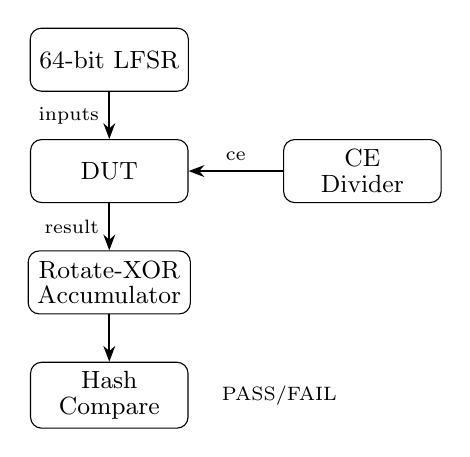
\begin{tikzpicture}[
  block/.style={draw, rounded corners, minimum width=2cm, minimum height=0.8cm, font=\small},
  arrow/.style={-{Stealth[length=2mm]}, thick},
  node distance=0.6cm
]
  \node[block] (lfsr) {64-bit LFSR};
  \node[block, below=of lfsr] (dut) {DUT};
  \node[block, below=of dut] (acc) {\shortstack{Rotate-XOR\\Accumulator}};
  \node[block, right=1.2cm of dut] (ce) {\shortstack{CE\\Divider}};
  \node[block, below=of acc] (cmp) {\shortstack{Hash\\Compare}};

  \draw[arrow] (lfsr) -- (dut) node[midway, left, font=\scriptsize] {inputs};
  \draw[arrow] (dut) -- (acc) node[midway, left, font=\scriptsize] {result};
  \draw[arrow] (ce) -- (dut) node[midway, above, font=\scriptsize] {ce};
  \draw[arrow] (acc) -- (cmp);

  \node[font=\scriptsize, right=0.3cm of cmp] {PASS/FAIL};
\end{tikzpicture}
\caption{CE-gated self-test harness.  The same structure runs twice:
first with CE divider = 256 (gold), then CE = 1 (test).  Hash mismatch
indicates timing failure.}
\label{fig:harness}
\end{figure}

The LFSR provides pseudo-random inputs with a 1-LUT critical path,
ensuring the harness itself does not limit the measurable frequency.
The harness ceiling was measured at $\sim$500~MHz (the LFSR-only
bypass passes at 500~MHz and fails at 525~MHz on the ECP5-25F
speed grade~6).

The NTSC CRT display module, active on a separate 25~MHz clock domain,
provides visual feedback: ``RUN'' during testing, ``PASS'' or ``FAIL''
upon completion.

% ===========================================================================
\section{Experimental Results}
\label{sec:results}
% ===========================================================================

\subsection{Platform}

All measurements were performed on a Colorlight 5A-75B v8.0 board
containing a Lattice ECP5-25F (speed grade 6) with 24K LUT4 and
28 DSP18 blocks.  The board provides a 25~MHz oscillator; all test
frequencies are generated via the EHXPLLL hard PLL.  Synthesis uses
Yosys (open-source) and place-and-route uses nextpnr-ecp5.  Area
is reported as LUT4 count with \texttt{-nowidelut} (pure 4-input
LUTs, no LUT combining).

\subsection{Comparison Libraries}

\textbf{Berkeley HardFloat}~\cite{hardFloat} provides IEEE~754
compliant arithmetic in recoded format.  For fair comparison, we
wrap each HardFloat core with \texttt{fNToRecFN} (input) and
\texttt{recFNToFN} (output) converters, measuring the full
IEEE-in/IEEE-out pipeline.  HardFloat core-only areas (without
converters) are: add 546, multiply 282, FMA 1344~LUT4.

\textbf{FPnew (CVFPU)}~\cite{fpnew} from ETH Z\"urich provides
native IEEE~754 arithmetic.  FPnew uses a unified FMA datapath
for all operations; standalone add and multiply are implemented by
hardcoding one FMA input.  We verified that Yosys constant
propagation optimizes away dead logic when inputs are hardcoded,
so FPnew add (825~LUT4) and multiply (574~LUT4) numbers reflect
optimized single-operation area.  The true three-input FMA is
2850~LUT4.  FPnew is pure-LUT (0~DSP) by design.

\subsection{Results: FPGA Target (with DSP)}

Table~\ref{tab:dsp} compares Spirix against HardFloat with DSP
blocks enabled.  This represents the typical FPGA deployment scenario.

\begin{table}[t]
\centering
\caption{Spirix vs.\ HardFloat --- FPGA with DSP (ECP5-25F, binary32)}
\label{tab:dsp}
\small
\begin{tabular}{@{}l rr r rr r@{}}
\toprule
 & \multicolumn{3}{c}{\textbf{Spirix}} & \multicolumn{3}{c}{\textbf{HardFloat+IEEE}} \\
\cmidrule(lr){2-4} \cmidrule(lr){5-7}
\textbf{Op} & LUT4 & DSP & MHz & LUT4 & DSP & MHz \\
\midrule
Add/Sub & 618 & 0 & 95 & 1050 & 0 & 88 \\
Multiply & 157 & 3 & 115 & 786 & 4 & 65 \\
FMA & 1128 & 3 & 63 & 2057 & 4 & 47 \\
\bottomrule
\end{tabular}
\end{table}

Spirix achieves 8\% higher Fmax on addition (95 vs.\ 88~MHz) with
41\% less area, 77\% higher Fmax on multiplication (115 vs.\ 65~MHz)
with 80\% less area and one fewer DSP, and 34\% higher Fmax on FMA
(63 vs.\ 47~MHz) with 45\% less area and one fewer DSP.

\subsection{Results: ASIC Target (no DSP)}

Table~\ref{tab:nodsp} compares Spirix against FPnew with all DSP
blocks disabled (\texttt{-nodsp}).  FPnew is inherently pure-LUT,
making this the natural 1:1 comparison for ASIC-style evaluation.

\begin{table}[t]
\centering
\caption{Spirix vs.\ FPnew --- No DSP (ECP5-25F, binary32)}
\label{tab:nodsp}
\small
\begin{tabular}{@{}l rr rr@{}}
\toprule
 & \multicolumn{2}{c}{\textbf{Spirix}} & \multicolumn{2}{c}{\textbf{FPnew}} \\
\cmidrule(lr){2-3} \cmidrule(lr){4-5}
\textbf{Op} & LUT4 & MHz & LUT4 & MHz \\
\midrule
Add/Sub & 618 & 95 & 825 & 74 \\
Multiply & 1750 & 95 & 2850 & 74 \\
FMA & 2768 & 53 & 2850 & 25 \\
\bottomrule
\end{tabular}
\end{table}

Without DSP blocks, Spirix wins on both area and speed across all
operations.  The FMA result is particularly significant: Spirix is
2.1$\times$ faster (53 vs.\ 25~MHz) while using 3\% less area
(2768 vs.\ 2850~LUT4).  Note that FPnew's add and multiply numbers
(825 and 574~LUT4 respectively) reflect Yosys constant propagation
of hardcoded FMA inputs; the true three-input FMA area of 2850~LUT4
is the fair comparison point since FPnew uses a unified FMA datapath.

\subsection{Static Timing vs.\ Silicon}

\begin{table}[t]
\centering
\caption{Static timing estimate vs.\ silicon-verified Fmax}
\label{tab:margin}
\small
\begin{tabular}{@{}l rrr@{}}
\toprule
\textbf{Module} & \textbf{Static} & \textbf{Silicon} & \textbf{Ratio} \\
\midrule
LFSR (harness only) & 205 & 500 & 2.4$\times$ \\
Spirix add/sub & 26 & 95 & 3.7$\times$ \\
Spirix multiply & 43 & 115 & 2.7$\times$ \\
Spirix FMA & 20 & 63 & 3.2$\times$ \\
HardFloat add & 25 & 88 & 3.5$\times$ \\
HardFloat multiply & 24 & 65 & 2.7$\times$ \\
HardFloat FMA & 16 & 47 & 2.9$\times$ \\
FPnew FMA & 17 & 25 & 1.5$\times$ \\
\bottomrule
\end{tabular}
\end{table}

Table~\ref{tab:margin} demonstrates that static timing analysis on the
ECP5 consistently underestimates achievable frequency by 1.5--3.7$\times$.
The ratio varies by design, making cross-design comparison using static
timing alone unreliable.  Silicon-verified measurements provide ground
truth.

\subsection{Pipeline Variants}

Both the adder and multiplier have two-stage pipelined variants that
further increase Fmax at the cost of one cycle of latency:

\begin{itemize}
  \item \textbf{Adder (pipe2)}: 148~MHz (vs.\ 95~MHz combinational),
        56\% improvement.
  \item \textbf{Multiplier (pipe2)}: 181~MHz (vs.\ 115~MHz combinational),
        57\% improvement, same 3~DSP.
\end{itemize}

These pipeline registers are CE-gated in the harness, ensuring proper
testing at full speed.

\subsection{IEEE f32 Accuracy}

To validate numerical correctness against the IEEE standard, we compare
Spirix addition against native Rust \texttt{f32} addition over 10 million
random input pairs.  Spirix fractions and exponents are converted to
IEEE binary32, the operation is performed in both systems, and results
are compared:

\begin{itemize}
  \item 99.97\% exact bit-for-bit match
  \item 0.025\% differ by exactly 1~ULP
  \item 0\% differ by more than 1~ULP
\end{itemize}

The 1-ULP differences arise from Spirix's slightly different rounding
boundary due to the absence of denormals and the single-zero property.
These are not errors---they represent valid rounding choices at the
boundary between the two systems' representable values.

% ===========================================================================
\section{Discussion}
\label{sec:discussion}
% ===========================================================================

\subsection{Why Two's Complement Wins}

The area and speed advantages stem from three architectural
simplifications:

\textbf{No sign-magnitude decomposition.}  IEEE adders must XOR the
sign bits with the subtract flag to determine effective operation,
then conditionally negate operands.  The two's complement adder simply
aligns and adds---the same integer adder handles all four sign
combinations.

\textbf{No exponent bias.}  IEEE multipliers compute
$e_{\text{result}} = e_a + e_b - \text{bias}$, requiring a subtraction
and wider intermediate.  Spirix computes $e_{\text{result}} = e_a + e_b$
directly.

\textbf{Simpler normalization.}  N-1 normalization guarantees the
product of two normal fractions needs at most a 1-bit left shift
(N-1 $\times$ N-1 $\to$ N-1 or N-2).  The FMA exploits this by
pre-aligning the addend in parallel with the multiply, since the
product exponent is known before the product fraction.

\subsection{Limitations}

The two's complement format does not support IEEE~754 special values
(NaN payload, signaling NaN, signed infinity).  Applications requiring
strict IEEE compliance cannot use this system.  The single ambiguous
exponent encodes overflow/underflow states that preserve sign
(``exploded''/``vanished'') but do not participate in further arithmetic
as IEEE infinities do.

The Karatsuba decomposition adds reconstruction overhead (+99~LUT4 with
DSP, where naive multiplication uses fewer LUTs but one more DSP block).
For designs where DSP blocks are abundant and LUTs are scarce, naive
multiplication may be preferable.

\subsection{Reproducibility}

All source code, synthesis scripts, and test harness configurations are
available in the project repository.  Results can be reproduced on any
Colorlight 5A-75B v8.0 board using the open-source Yosys/nextpnr
toolchain.  The build command for a given frequency:
\begin{verbatim}
SEED=4 bash fpga/scripts/build_ntsc.sh \
  <freq_mhz> --program
\end{verbatim}

% ===========================================================================
\section{Related Work}
\label{sec:related}
% ===========================================================================

\textbf{TMS320C3x} (Texas Instruments, $\sim$1988)~\cite{tms320c3x} is
the closest historical precedent: its floating-point format uses a two's
complement mantissa with an unbiased two's complement exponent---the same
core representation as our system.  However, the TMS320C3x was a
proprietary DSP with no published area or frequency comparisons against
IEEE~754 implementations on equivalent hardware.  The format was
abandoned in later TI generations in favor of IEEE compliance.

\textbf{Boldo and Daumas}~\cite{boldo2003} formally verified properties
of two's complement floating-point notations using the Coq proof
assistant, referencing the TMS320C3x addition flowchart.  Their work
establishes theoretical correctness properties (including an extension
of Sterbenz's theorem) but does not address hardware implementation or
comparison.

\textbf{LOCOFloat}~\cite{locofloat} (2020) uses two's complement for
both significand and exponent in an FPGA-targeted format optimized for
hardware-in-the-loop simulation.  LOCOFloat focuses on area reduction
via ``soft normalization'' (relaxed normalization constraints) rather
than on arithmetic correctness properties or comparison against
established IEEE libraries.

\textbf{Berkeley HardFloat}~\cite{hardFloat} implements IEEE~754
arithmetic using a recoded internal format that simplifies normalization
detection.  The recoded format adds a leading bit to the exponent,
requiring input/output converters for IEEE interoperability.  HardFloat
targets ASIC flows and has been used in RISC-V cores including BOOM
and Rocket.

\textbf{FPnew / CVFPU}~\cite{fpnew} from ETH Z\"urich provides a
configurable IEEE~754 floating-point unit using a unified FMA datapath.
It supports multiple precision formats and rounding modes.  FPnew is
used in the PULP (Parallel Ultra-Low-Power Processing) platform and
the CVA6 RISC-V core.  Its pure-LUT design (no DSP inference) makes
it suitable for ASIC targets.

\textbf{Posit arithmetic}~\cite{posit} represents an alternative to
IEEE~754 with tapered precision, but uses sign-magnitude representation
and requires variable-length decoding of the regime field, introducing
different implementation challenges.

To our knowledge, no prior work presents a silicon-verified comparison
of two's complement floating-point arithmetic against established IEEE~754
libraries on identical hardware.  The TMS320C3x demonstrated the format's
viability in commercial silicon but predated both HardFloat and FPnew
by decades; Boldo and Daumas provided formal foundations but no
implementation data; LOCOFloat targeted a different design point
(relaxed normalization, no FMA).  We conducted an extensive literature
search and found no published head-to-head area and frequency comparison
between two's complement and IEEE~754 floating-point implementations.

% ===========================================================================
\section{Conclusion}
\label{sec:conclusion}
% ===========================================================================

We have demonstrated that two's complement floating-point arithmetic
achieves both higher operating frequency and lower area than IEEE~754
implementations on FPGA silicon.  The architectural simplifications
enabled by eliminating sign-magnitude decomposition, exponent bias,
and complex special-value handling translate directly into measurable
hardware advantages across all three fundamental operations (add,
multiply, FMA).

The CE-gated self-test methodology provides a rigorous alternative to
static timing analysis for FPGA frequency characterization, consistently
revealing 2--3.7$\times$ higher achievable frequencies than static
estimates predict.

Future work includes pipelined FMA variants for higher throughput,
combined division/square-root units, and ASIC synthesis targeting
standard cell libraries for area and power comparison at advanced
process nodes.

% ===========================================================================
% References
% ===========================================================================

\begin{thebibliography}{9}

\bibitem{tms320c3x}
Texas Instruments, ``TMS320C3x User's Guide,'' SPRU031F, 1997.
Two's complement mantissa with unbiased two's complement exponent.

\bibitem{boldo2003}
S.~Boldo and M.~Daumas, ``Properties of Two's Complement Floating
Point Notations,'' \emph{International Journal on Software Tools for
Technology Transfer}, vol.~5, no.~2--3, pp.~237--246, 2003.

\bibitem{locofloat}
A.~Sanchez, A.~de~Castro, M.~S.~Mart\'inez-Garc\'ia, and J.~Garrido,
``LOCOFloat: A Low-Cost Floating-Point Format for FPGAs: Application
to HIL Simulators,'' \emph{Electronics}, vol.~9, no.~1, p.~81, 2020.

\bibitem{hardFloat}
J.~Hauser, ``Berkeley HardFloat,''
\url{https://github.com/ucb-bar/berkeley-hardfloat}, 2019.

\bibitem{fpnew}
S.~Mach, F.~Zaruba, and L.~Benini, ``FPnew: An Open-Source
Multi-Format Floating-Point Unit Architecture for Energy-Proportional
Transprecision Computing,'' \emph{IEEE Transactions on Very Large Scale
Integration (VLSI) Systems}, vol.~29, no.~4, pp.~774--787, 2021.

\bibitem{posit}
J.~Gustafson and I.~Yonemoto, ``Beating Floating Point at its Own
Game: Posit Arithmetic,'' \emph{Supercomputing Frontiers and
Innovations}, vol.~4, no.~2, 2017.

\end{thebibliography}

\end{document}
